% INTRODUCTION

% \todo[inline,color=yellow!40]{The introduction is one of the most important pieces of your thesis.  Here is a place for you to introduce the problem(s) on which you have worked and place them in the larger context of your field. You should aim to ensure that this section is completely understandable to virtually anyone - and certainly anyone with a sophomore-level grasp of physics.  Presumably, this will include references to the literature.
% \\
% In addition to setting your work into context, a second good idea for your introduction is to give a short outline for what the rest of your thesis will discuss.  This is often done in the closing paragraph(s) of the introduction with sentences like ``In the following chapters \ldots " and ``Chapter 2 discusses \ldots"  Tremendous detail is not required in this outline, but rather just a brief road map for the rest of the document.}

% synchrtron radiation section is the intro
Synchrotron radiation was first observed by General Electric in Schenectady, New York \cite{firstSynchrotronRadPaper}. Initially just a side effect of particle accelerator experiments, it has since grown to be an important and powerful source of high-energy electromagnetic radiation for structural determination. Compared to lab-scale x-ray generation for diffraction experiments, arguably the most important benefit of synchrotron radiation is its high brilliance. Synchrotron radiation creates a highly collimated beam of photons characterized by small divergence and spatial coherence. Additionally, synchrotron radiation is tunable across a wide spectrum (microwaves to hard X-rays) and capable of high flux, useful for short time-scale-dependent experiments or weak scatterers. Synchrotron radiation can be produced in a pulsed structure. Importantly, the incoming photons are highly polarized, either linearly or circularly, depending on where the measurement system lies with respect to the plane of the synchrotron. The advent of a technique to manufacture such a high-quality source of x-rays allowed for new, advanced methods of x-ray absorption spectroscopy, and the two fields were developed in parallel. 

\section{X-ray Absorption Spectroscopy}
X-ray absorption spectroscopy measures the absorption of high-energy photons by a sample as a function of energy \cite{gardenghi2012synchrotron}. The attenuation, or change in transmitted light intensity as a result of inelastic processes, is characterized by the Beer-Lambert Law (\ref{BeerLambert}). For an incident beam of intensity $I_0$, the transmitted intensity after interacting with an attenuation
coefficient of $ \mu $ and a sample of thickness $ x $ is: 

\begin{equation}
    \label{BeerLambert}
    I = I_0 e^{-\mu x}
\end{equation}

Above the absorption edge, the condensed state has characteristic absorption jumps where the incident photon's energy matches the binding energy of a core electron. At this energy, nearly all the photon's energy is absorbed by the core electron, resulting in the characteristic absorption-edges first observed in 1920 \cite{fricke1920, hertz1920ueber}.

In experimental setups, particular energy photons are selected from the broad spectrum of synchrotron radiation via a pair of monochromaters. The primary monochromater is a crystal with interplanar spacing, $ d $, chosen specify to satisfy the Bragg equation \ref{Bragg}, relecting photons of wavelngth, $ \lambda $ at angle $ \theta $.  

\begin{equation}
    \label{Bragg}
    n\lambda = 2d\sin(\theta)
\end{equation}

The secondary monochromater removes higher order harmonics that satisfy the Bragg equation $ (2\lambda, 3\lambda etc.). $ Different wavelngths of light can be selected by changing the angle. In the XAFS setup, two ionization chambers are used to measure the incident and transmitted light intensity. For any study, the absoprion spectrum for a reference sample is also measured to calibrate the energy scale.


\subsection{XAFS}
X-ray Absorption Fine-Structure (XAFS) spectroscopy refers to the study of absorption spectra created from high-intensity x-ray interactions. As the energy of the incident radiation increases, the photon's energy will eventually match the binding energy of a core-level electron. As a result, an ``edge'' in the spectrum will be observed. The location of these edges depends on the chemical and physical structure, as well as the electronic and vibrational states of the material. Absorption edges are like fingerprints used to identify elements, distinguish oxidation states, and even probe short-range order from the characteristic peaks and oscillations in the spectrum. XAFS spectroscopy can be performed on virtually any stable element since all atoms contain core-level electrons. Although a high-quality source of x-rays such as synchrotron radiation is required for the analysis, the ubiquity and utility of XAFS spectroscopy has made it an indispensable technique in fields such as materials biology, chemistry, and materials science \cite{rehrXAFS2000review} \cite{newville2014fundamentals}.

% \textit{absorption edges like fingerprints to identify elements. in 1920 Frische and Hertz observed peak shape, and 40 years later it was learned that this shape can be used to probe the short-range order.1971 e.a. Sterne expalin this effect. Fermi's golden rule. The inelastic interactions of the photon are related to characteristic energies. When the photon energies match the energy difference from the core-electron state to the first unoccupied level, the photon can be fully absorbed (before that only partially absorbed.)}
The XAFS equation is 
\begin{equation}
    \label{XAFS}
    \chi = \dfrac{ \mu(E)- \mu_{0}(E)  }{  \mu_{0}(E) - \mu_{ b  }(E)  } 
\end{equation}

\noindent where $\mu$ is the measured absorption, $ \mu_0 $  is the ``atomic'' absorption due to .... specific electrons, and $ \mu_b $ 
is the absorption of other processes \cite{klementev2000xafs}, typically approximated with the Victoreen polynomial (\ref{Victoreen}).

\begin{equation}
    \label{Victoreen}
    \mu_b(E) = aE^{-3} + bE^{-4}
\end{equation}

\noindent The coefficients $ \alpha $ and $ \beta $ can be found via a simple regression on a sprectrum measured at pre-edge energies \cite{klementev2000xafs}. 

The XAFS spectrum is typically divided into two regions of study: the area near the first absorption peak ---XANES, and the area after ---EXAFS. XANES has a strong sensitivity to the oxidation state and coordination
chemistry of the absorbing atom, while the EXAFS
can be used to determine the bond lengths, coordination numbers, and atomic species of the absorbing atom's neighbors.
% "The most difficult procedure in extracting of XAFS from the measured absorption is the construction of μ0 since
% one cannot definitely distinguish the environmental-born part of absorption from the atomic-like one. \cite{klementev2000xafs}"

\subsection{EXAFS}
Beyond the edge of the absorption spectrum lies the Extended X-ray Absorption Fine Structure (EXAFS) region. The spectral shape of this domain is determined by the multiple scattering of the photoelectron, interference of the incoming and outgoing waves of the photon, and electronic energy level splitting of the local structure. The oscillations in the EXAFS region are extremely sensitive to local bond lengths, coordination numbers, and atomic species of the surrounding elements.


\subsubsection{EXAFS Data Reduction}
To prepare the absorption data for fitting (data reduction), several steps must be performed. First the pre-edge background must be removed using the Victoreen formula (\ref{Victoreen}) or an alternative polynomial. Next, the atomic background, $ \mu_0(E) $  is removed and the absorption measured absorption is normalized accordingly. This is a non-trivial process, as the absorption coefficient is not that of a single, isolated atomic absorber; instead, it represents that of an atom and its surrounding neighbors. High order spline fittings must be used to remove the low frequency, immeasurable oscillations due to photoelectron scattering with nearby valence electrons. For EXAFS Fitting, the EXAFS function is often transformed into k-space, and Fourier transformed into a radial distribution-like function via (\ref{red-exafs}) \cite{exafsbook}.

\begin{equation}
    \label{rdf-exafs}
    \widetilde{\chi}(r) = \frac{1}{2\pi} \int_{0}^{\infty }  k^n \chi(k) e^{2ikr} dk
\end{equation}

Alternatively, one can convert the wave to R-space, which is what Artemis and Athena, two of the most common EXAFS fitting software, do.

\subsubsection{The EXAFS Equation}
With the data reduction complete, a multi-parameter fitting can be performed via the EXAFS equation. This equation is an approximation based principally on the many-body Fermi golden rule (\ref{FermisGoldenRule}).

\begin{equation}
    \label{FermisGoldenRule}
    % Fermi's GOlden Rule for a one e- approximation
    \mu(E) \varpropto \sum_{f}^{E_f > E_F} \left\lvert \left\langle f \lvert H_{int} \rvert i \right\rangle \right\rvert ^2 \delta (E - E_F - Ef)  
\end{equation}

\noindent Fermi's golden rule describes the probability of a transition in state occurring. Here (\ref{FermisGoldenRule}), $ \mu(E) $ is the absorption coefficient, $ f $ and $ i $ are the final and initial states of the photoelectron, respectively. $ H_{int} $ is the matter-light interaction operator, and the delta function ensures conservation of energy. The summation over all enegy values approximates the many-bodied problem as a single particle theory. 

At energies above the core electron binding energy, excess energy is transferred to the photoelectron, which may then undergo multiple scattering with the surrounding atoms. The final wavefunction of the photoelectron is the superposition of the outgoing photoelectron and the scattered wave. EXAFS only takes into account the local region around the absorber at a distance $ r_j $  from the backscattering atom.

\begin{equation}
    \label{superposition_Exafs}
    \chi(k) \approx F_j(k) \dfrac{\sin[2kr_j + \phi_{ij}(k)]}{2r_j^2}
\end{equation}

The above equation (\ref{superposition_Exafs}) describes the EXAFS signal for only one backscattering atom. For a system with many atoms, one must sum over all the backscattered waves. To account for the inevitable variation in bond lengths, the Debye-Waller factor $ \sigma_j $ is introduced; this describes the standard deviation in bond-length of the sample.\footnote{Note, this differs from the Debye-Waller factor used for x-ray absorption, which describes the broadening of a diffraction peak due to variations in inter-planar spacing \cite{DW-diffraction}}. The lifetime of the photoelectron's excited state is taken into account by introducing an exponential term to account for the mean-free-path, $ e^{-2r_j/\lambda} $. Combining all this information with an amplitude correction factor of $ S_0 $, we arrive at the EXAFS equation (\ref{ExafsFormula}. 

\begin{equation}
    \label{ExafsFormula}
    \chi(k) = \sum_j \frac{N_j}{kr_j^2}F_j(k)e^{-2\sigma_j^2k^2}e^{-\tfrac{2r_j}{\lambda(k)}}\sin[2kr_j + \phi_{ij}(k)]
\end{equation}

Although popular, the EXAFS equation is still a first-order approximation with assumptions and limitations. For example, the fitted disorder parameter, the Debye-Waller factor, explicitly assumes a Gaussian distribution of nearest-neighbor bond length distances. Other more accurate but computationally intensive alternatives are increasing in popularity. Such alternatives include molecular dynamics, reverse Monte Carlo simulations and neural networks \cite{lin2020machine} \cite{timoshenko2018neural}.

\subsection{XANES}
The XANES region, or the near-edge region, encodes the chemical and electronic structural information of the sample within its shape. The XANES shape reflects the lower energy photons which scatter much more strongly than in the EXAFS region. XANES also has the advantage of a higher signal-to-noise ratio than the subtle interference-determined oscillations found in EXAFS. While there is an ``EXAFS Equation,'' there is no ``XANES Equation'' equivalent; however, this does not mean that there is no structural information encoded in the XANES, only that the theory is underdeveloped. Mainly, the strong errors in potential and many-body effects limit the development of a ``XANES equation.'' 

With the recent explosion in the popularity of machine learning, the investigation of the XANES latent space has become a topic of modern research is. In other words, how much information is encoded in XANES?

Recent work at Brookhaven National Lab \cite{Timoshenko2017} has shown that it is possible for a model to learn structural descriptors from the XANES spectrum. Specifically, their method enables the decoding of XANES spectra to obtain the coordination number of metallic nanoparticles. In this 2017 paper, the group trained an artificial neural network (ANN) to recognize a relationship between the nanoparticle structure and the XANES spectrum. Once trained, the ANN is used to ``invert'' an unknown spectrum to obtain the corresponding structural descriptors of the catalyst. These descriptors, the coordination numbers, are used to calculate the number of shells (nanoparticle size) and shape (Archimedian solid) of the sample. While this model can determine the structure of nanoparticles from XANES ---a feat previously only possible with the full EXAFS spectrum ---it still has one major limitation: the ANN does not predict the disorder of the structure. The bond-length disorder is known to be an important descriptor for catalyst \cite{catalyst-strain-dependence} \cite{co-strain-effects}.

\begin{figure}
    \centering
    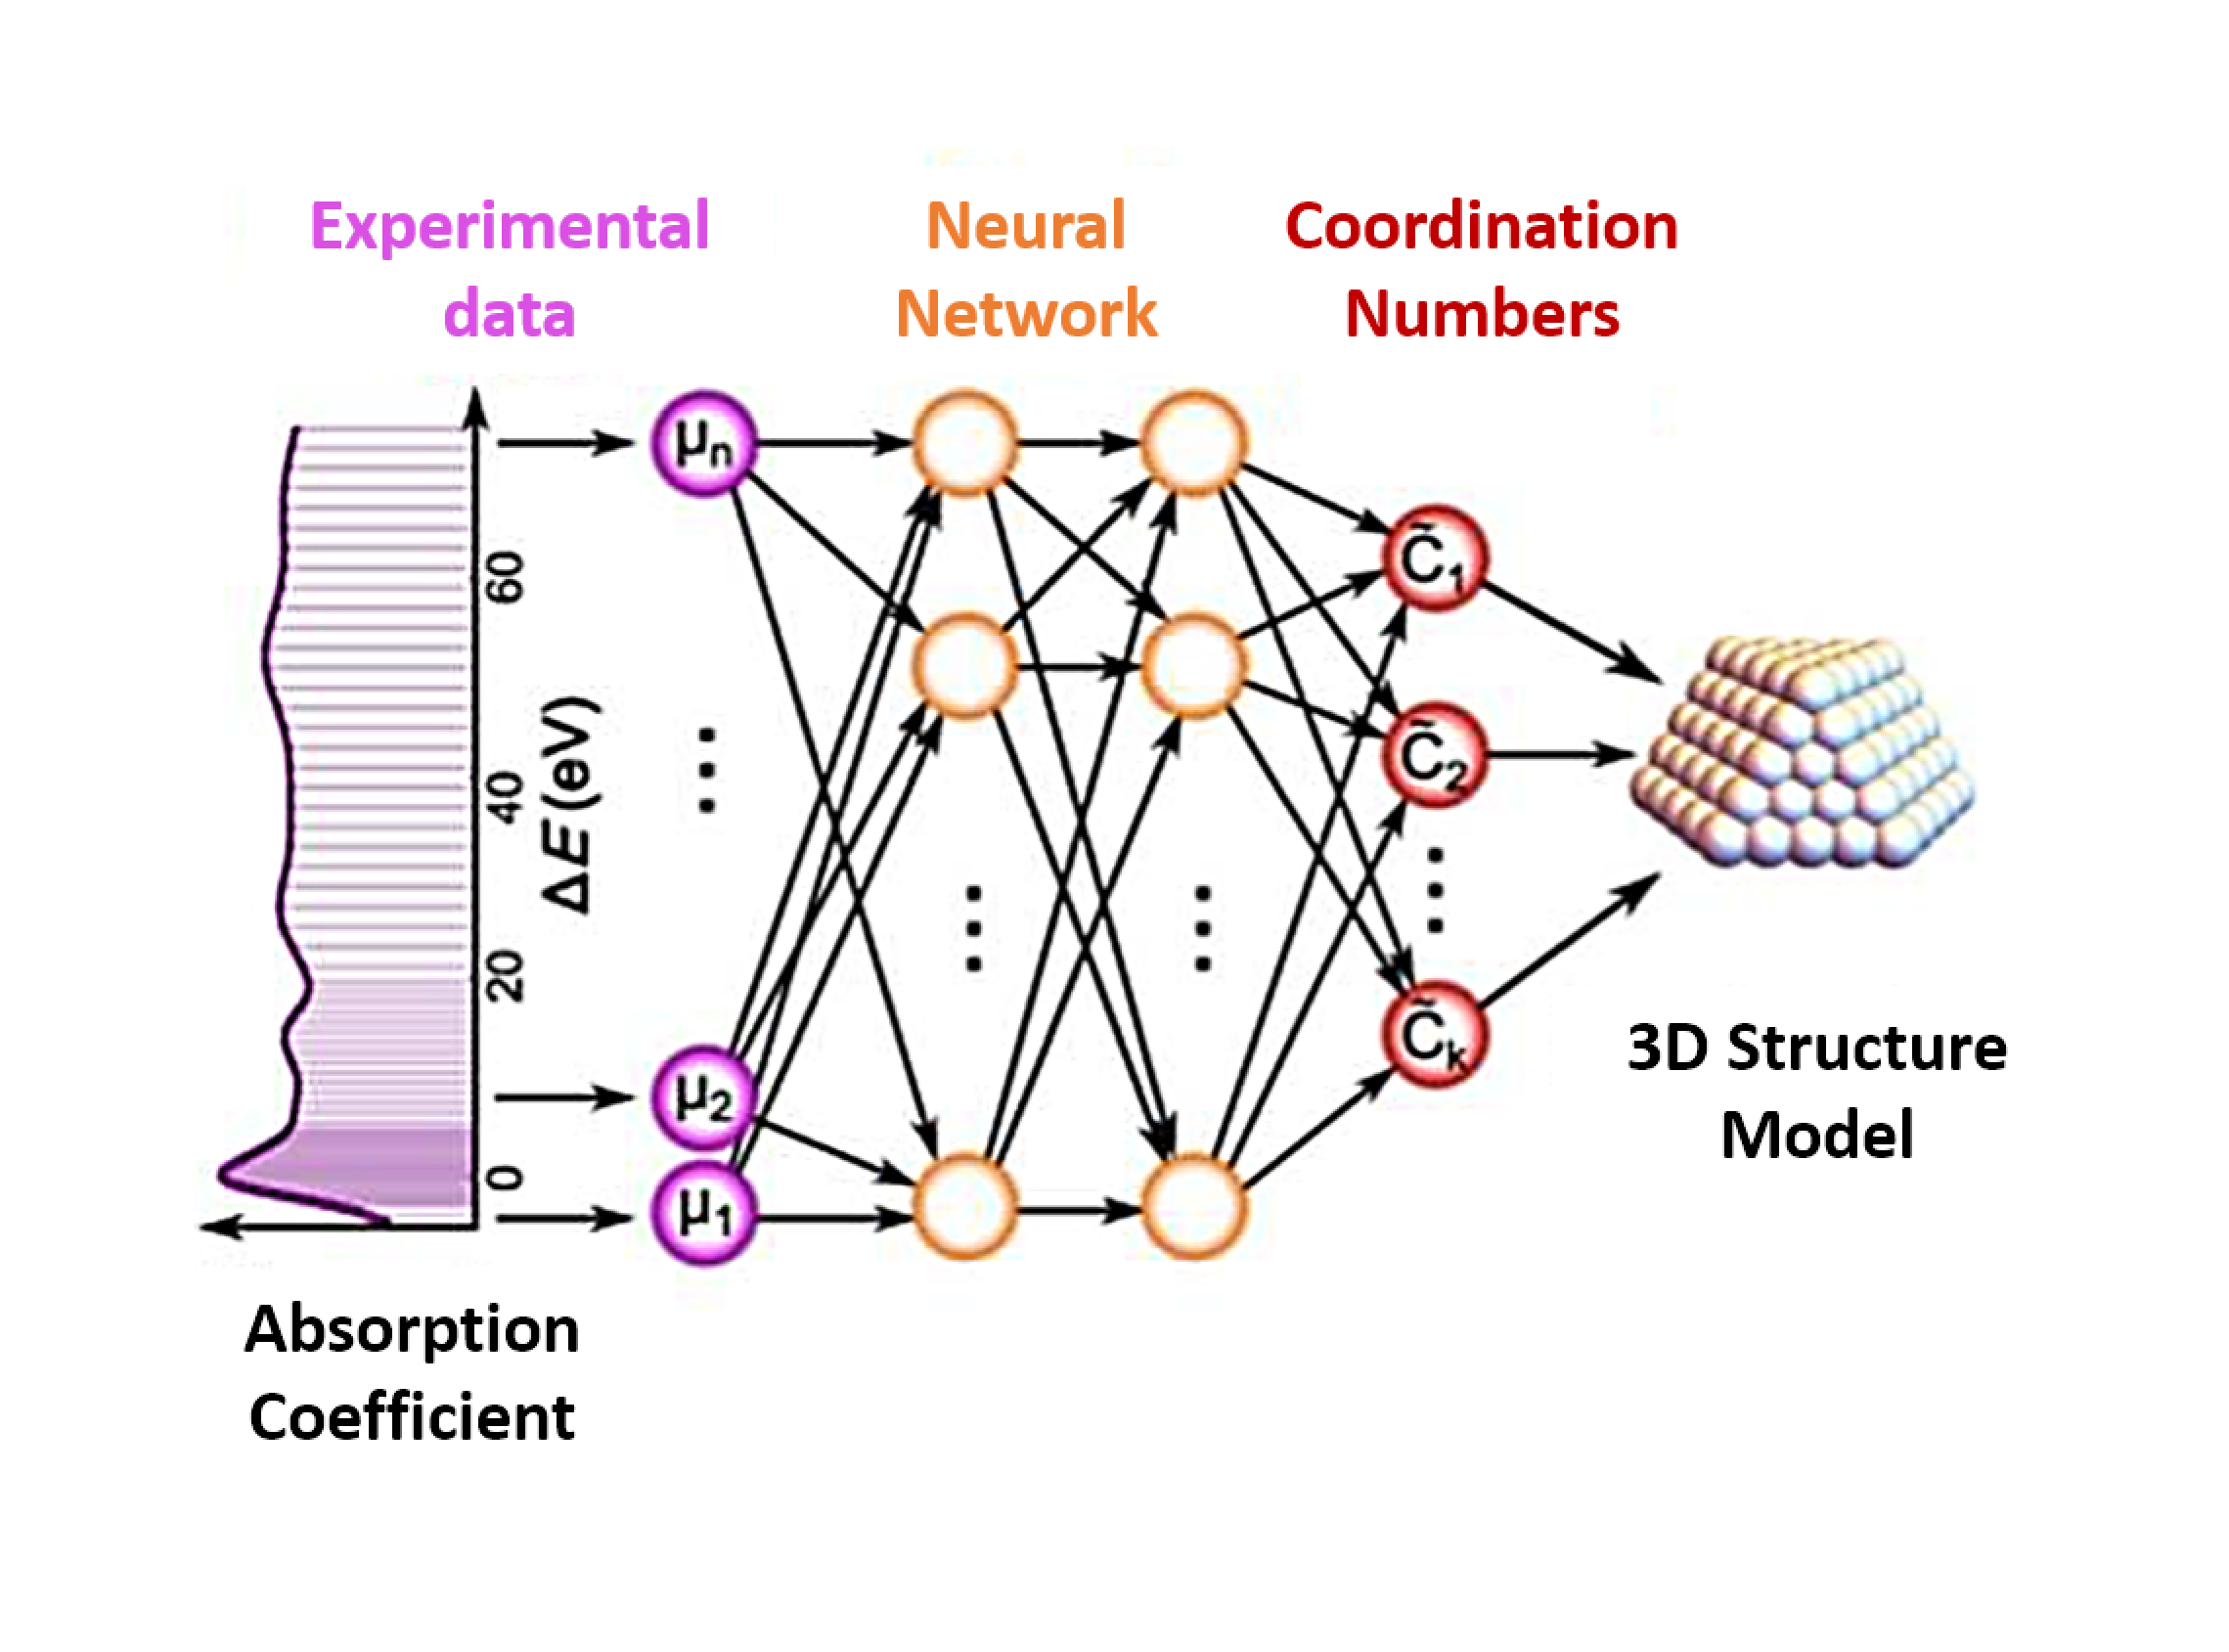
\includegraphics[width=.75\linewidth]{Chapters/Figures/placeholderFrenkel2017.png}
    \caption[ANN Metallic Nanoparticles]{From \cite{Timoshenko2017}, the neural netowrk is trained to take a XANES spectrum from a metallic nanoparticle, and predict the coordination number of the structure. This coordination number of nanoparticles is a known discriptor, which allows for easy calculation of the the nanoparticle's size and shape.}
\end{figure}

\section{Diagram for collecting experimental XAFS data???}

\section{Goals of the Thesis and Approach}
Building of the previous work \cite{Timoshenko2017}, the goal of this thesis is comprised of two parts: first, determine whether bond-length information is encoded in the XANES spectrum; and second, utilize machine learning to predict the bond-length disorder of metallic nanoparticles from a XANES spectrum. As with the 2017 paper \cite{Timoshenko2017}, the work is conducted with gold (Au) nanoparticles, in part to expand on the previous paper, and in part due to the access to the relevant experimental data. Machine learning requires a substantial amount of training data, far more than could be experimentally obtained. Consequently, we will rely on absorption simulation software to create the training data, a collection of XANES spectra for Au nanoparticles with known disorder. Finally, once the network is trained, the network must be modified to abstract to experimental data to compenstate for the systematic differences between the simulation and experimental data.

\section{Outline of the Thesis}
Often the most time-intensive part of any machine learning-based project is the process of collecting and preprocessing the data. Chapter 2 is dedicated entirely to the process of generating XANES spectra via simulations. Next, a solid foundational understanding of machine learning is important in understanding the approach. All machine learning terms present in later chapters are defined here.  Chapter 4 describes the exact model architecture and results of the training process. Further discussions and future work are included in chpater 5. \textit{Appendix A includes a description of the main Python script written for this thesis and necessary for replicated the work. The files can be obtained upon request by contacting the author.}
% Building off the historical context of measuring disordered nanoparticles in XANES spectra, this thesis begins with an in-depth description of 
